\subsection{$R$-矩阵作用}%
\label{sub:R-matrix action}

21 世纪初，Givental 发现了公理化枚举理论的一个显著性质，即可以利用满足如下性质的矩阵 $R(z) = R_0 + R_1 z + R_2 z^2 + \cdots \in \Hom(V, V')\ps{z}$ 的作用来变换 CohFT
\[ R^*(-z) R(z) = \mr{Id}_V. \]
传统上，文献要求 $V = V'$ 且 $R_0 = \mr{Id}$，但 MSP 群已经去除了这一限制，并且也允许 $\dim V < \dim V'$。

为了定义 $R$ 在 $V$ 上的 CohFT $\Omega$ 上的作用，我们需要回顾 $\Mbar_{g,n}$ 的一些组合结构。对曲线 $C\in \Mbar_{g,n}(\C)$，可以考虑 $C$ 的对偶图，它由顶点、边和腿（leg）组成，定义如下：
\begin{itemize}
    \item 顶点对应于 $C$ 的不可约分支，并由一个非负整数标记，即其亏格；
    \item 边对应于 $C$ 的结点（特别地，我们允许环）；
    \item 腿对应于标记点。
\end{itemize}
任何作为稳定曲线的对偶图出现的图都称为 \textit{稳定图}。

\begin{figure}[htpb]
  \centering
  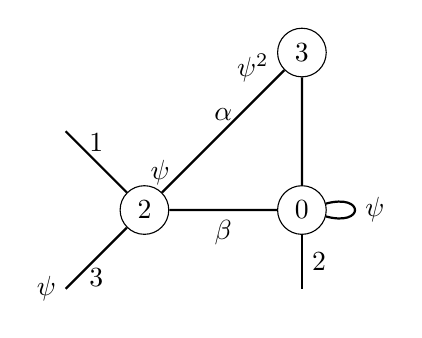
\begin{tikzpicture}[scale=1,transform shape,every loop/.style={}]
    \node[circle,draw] (A) at (0,0) {$2$};
    \node[circle,draw] (B) at (2,2) {$3$};
    \node[circle,draw] (C) at (2,0) {$0$};
    \draw[thick] (A) -- node[above]{$\alpha$} (B) -- (C) -- node[below]{$\beta$} (A);
    \draw[thick] (A) -- node[below]{$3$} (-1,-1);
    \draw[thick] (A) -- node[above]{$1$} (-1,1);
    \draw[thick] (C) -- node[right]{$2$} (2,-1);
    \draw[thick] (C) edge[loop right] node[right] {$\psi$} (C);
    \node[anchor=east] at (-1,-1) {$\psi$};
    \node[anchor=east] at (1.7,1.8) {$\psi^2$};
    \node[anchor=south] at (0.2,0.2) {$\psi$};
  \end{tikzpicture}
  \caption{$\ol{\mc{M}}_{7,3}$ 中的一个稳定图及其相伴重言类。该稳定图描述了映射
    $\ol{\mc{M}}_{2,4} \times \ol{\mc{M}}_{3,2} \times \ol{\mc{M}}_{0,5} \to \ol{\mc{M}}_{7,3}$ 的像。}
  \label{fig:stablegraph}
\end{figure}

作用在 CohFT 上的第一类作用是平移作用。设 $T \in V\ps{z}$。对 CohFT $\Omega$，我们定义
\[ (T\Omega)_{g,n}(\bv) \coloneqq \sum_m \frac{1}{m!} p_* \Omega_{g,n+m}(\bv, T,\ldots,T) \]
只要该无穷和有意义。

\begin{exm}
    若 $\Omega^X$ 是光滑射影簇 $X$ 的 GW CohFT，且 $\tau \in H^2(X)$ 是一个除子类，则该无穷和有意义，我们可以定义 $X$ 的平移后的 GW CohFT $\Omega^{X,\tau}$。例如，若 $X$ 是五次三维簇且 $\tau = \frac{I_1}{I_0} H$，则平移到 $\tau$ 等同于镜像映射 $q \mapsto Q(q) = q e^{\frac{I_1}{I_0}}$。
\end{exm}

第二类作用是本节开头所述矩阵 $R$ 的作用。设 $G_{g,n}$ 表示所有亏格为 $g$、带有 $n$ 条腿的稳定图的集合。我们定义
\[ (R\Omega)_{g,n} \coloneqq \sum_{\Gamma \in G_{g,n}} \frac{1}{\ab|\Aut \Gamma|} \on{Cont}_{\Gamma}, \]
其中 $\on{Cont}_{\Gamma}$ 由如下构造定义：
\begin{itemize}
    \item 在第 $i$ 条腿上放置映射 
        \[ R(-\bar{\psi}_i)^* \in \Hom(V',V) \ps{\bar{\psi}_i}; \]
    \item 在每条边上放置双向量
        \[ V(\bar{\psi}_1, \bar{\psi}_2) \coloneqq \sum_{\mu} \frac{e_{\mu} \otimes e^{\mu} - R(-\bar{\psi}_1)^* e_{\mu} \otimes R(-\bar{\psi}_2)^* e^{\mu}}{\bar{\psi}_1 + \bar{\psi}_2}; \]
    \item 在每个顶点上放置线性映射
        \[ \Omega_{g_v, n_v} \colon V^{\otimes n_v} \to H^*(\Mbar_{g_v, n_v}); \]
    \item 最后，我们考虑沿粘合态射 $\prod_v \Mbar_{g_v, n_v} \to \Mbar_{g,n}$ 在上同调中的前推。
\end{itemize}

\begin{defn}
    设 $R$ 如上。我们定义平移
    \[ T_R \coloneqq z (\1 - R(-z)^* \1') \in z V\ps{z}. \]
    只要其有意义，我们就定义
    \[ R.\Omega \coloneqq RT\Omega. \]
\end{defn}

\begin{thm}[Chang-Guo-Li {\cite[Theorem~2.7]{CGL2026}}]
    假设我们取系数在 $\C\ps{q}$ 中。那么若
    \[ T_R \in z^2 V \ps{z} + zq V \ps{z}, \]
    则 $R.\Omega$ 是一个良定义的 CohFT。此外，若 $\dim V = \dim V'$，则 $\1'$ 是 $R.\Omega$ 的单位。
\end{thm}

我们想就 $R_0 \neq \mr{Id}$ 时的平移作用多作一些说明。为简单起见，假设 $V = V'$ 且对某个常数 $c$ 有 $R_0 \1 = c \cdot \1$。于是我们令 $\tilde{T}_R \coloneqq z( \1 - c R(z)^{-1} \1)$，并利用膨胀子方程计算
\begin{align*}
    T_R \Omega_{g,n}(\bv) &= \sum_{m=0}^{\infty} \frac{1}{m!} p_*\Omega_{g,n+m}(\bv, T_R, \ldots, T_R) \\
    &= \sum_{k,\ell \geq 0} \frac{1}{k!\ell!} p_* \Omega_{g,n+k+\ell}(\bv, ( (1-c^{-1})\1 \cdot \psi )^{\otimes k}, ( c^{-1} \tilde{T}_R )^{\otimes \ell}) \\
    &= \sum_{k,\ell \geq 0} \frac{(1-c^{-1})^k \cdot c^{-\ell}}{\ell!} \binom{2g-2+n+k+\ell-1}{k} p_* \Omega_{g,n+\ell}(\bv, \tilde{T}_R^{\otimes \ell}) \\
    &= \sum_{m=0}^{\infty} \frac{c^{2g-2+n}}{m!} p_* \Omega_{g,n+m}(\bv, \tilde{T}_R, \ldots, \tilde{T}_R)
\end{align*}
只要上式有意义。


\subsection{重构定理}%
\label{sub:Reconstruction theorem}

回顾每个 CohFT 都定义一个弗罗贝尼乌斯代数。若相应的弗罗贝尼乌斯代数是半单的，我们称该 CohFT 是 \textit{半单} 的。

\begin{thm}[Teleman {\cite{Teleman2012}}]%
\label{thm:teleman}
    设 $\Omega$ 是带平坦单位的半单 CohFT，$\omega$ 为其拓扑部分。则存在唯一的
    \[ R = \mr{Id} + R_1 z + \cdots \in \End(V)\ps{z} \]
    使得
    \[ \Omega = R.\omega. \]
\end{thm}

\begin{exm}
    回顾前文的 Hodge 丛 CohFT。它由公式
    \[ \Omega^{\E}_{g,n} = c(\E) = 1 + \lambda_1 + \cdots + \lambda_g. \]
    给出。取零次部分，可见 $\omega^{\E}$ 是一点的 GW CohFT。利用 Mumford 的计算
    \[ \ch(\E) = g + \sum_{k=1}^{\infty} \frac{B_{2k}}{(2k)!}\ab(\kappa_{2k-1} + \frac{1}{2}\iota_*\sum_{i=0}^{2k-2} \bar{\psi}_1^{i} (-\bar{\psi}_2)^{2k-2-i}), \]
    其中 $\kappa_{m} = p_* \bar{\psi}_{n+1}^{m+1}$，$B_{2k}$ 是 Bernoulli 数，$\iota$ 是边界在相差一个 $2:1$ \'etale 覆盖意义下的嵌入，以及对任意向量丛 $E$ 的公式
    \[ c(E) = \exp \ab(-\sum_k (-1)^k (k-1)!\ch_k(E)) \]
    （或直接使用量子 Riemann-Roch 定理\footnote{Coates-Givental 中有一个符号错误，并已传播到后续的文献中。}），我们得到 $R$-矩阵
    \[ R(z) = \exp\ab( \sum_{k=1}^{\infty} \frac{B_{2k}}{2k(2k-1)} z^{2k-1}) = 1+\frac{1}{12}z + \cdots. \]

    作为一个合理性检验，我们将用 $R$-矩阵计算 $\Omega_{1,1}^{\E}$。首先，我们考虑~\Cref{fig:03graphloop} 中的稳定图。
    \begin{figure}[htpb]
    \begin{center}
    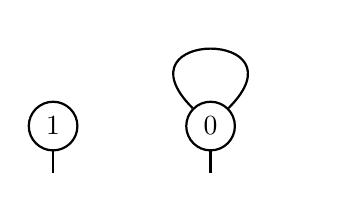
\begin{tikzpicture}[scale=1, transform shape, every loop/.style={}]
    \node[circle,draw=black,thick] (B) at (-1,0) {$1$};
    \draw[-,thick] (B) -- (-1,-0.6);
    \node[circle,draw=black,thick] (A) at (1,0) {$0$};
    \draw[-,thick] (A) -- (1,-0.6);
    \path[every node/.style={font=\sffamily\small},thick]
        (A)   edge[loop] (A);
    \end{tikzpicture}
    \end{center}
    \caption{$g=1, n=1$ 的稳定图}%
    \label{fig:03graphloop}
    \end{figure}
    第一个图 $\Gamma_1$ 给出贡献
    \begin{align*}
        \Cont_{\Gamma_1} &= T\omega_{1,1}^{\E}(R(z)^{-1}\1) \\
        &= \omega_{1,1}^{\E}(R(z)^{-1}\1) + p_* \omega_{1,1}^{\E}(R(z)^{-1}\1, T_R(z)).
    \end{align*}
    利用公式 $B_2 = \frac{1}{6}$ 以及 $\dim \Mbar_{1,1} = 1$ 的事实，上式变为
    \[ 1 - \frac{1}{12}\psi_1 + \frac{1}{12} \kappa_1. \]
    第二个图没有尾部贡献，因为 $\dim \Mbar_{0,3} = 0$。边贡献的常数项是 $\frac{1}{12}$，因此考虑自同构并前推到 $\Mbar_{1,1}$，我们得到
    \[ \Cont_{\Gamma_2} = \frac{1}{12} \Delta, \]
    其中 $\Delta$ 表示边界除子（带有正确的叠结构）。由于此时 $\psi_1 = \kappa_1$，我们得到
    \[ 1+\lambda_1 = 1 + \frac{1}{12}(\kappa_1 - \psi_1 + \Delta) = 1 + \frac{1}{12} \Delta. \]
\end{exm}




\subsection{算符形式与几何量子化}%
\label{sub:Operator formalism and geometric quantization}

我们回到 Givental 的辛形式。它对某些计算更为方便，但事实上它与我们之前的理论相同，至少在我们想要计算生成函数时是如此。回顾我们在 $V$ 上有弗罗贝尼乌斯流形结构，并考虑带辛形式
\[ (\mbf{f}(z), \mbf{g}(z)) \coloneqq \on{Res}_{z=0} \eta(\mbf{f}(-z), \mbf{g}(z)). \]
的向量空间 $\mc{V}\coloneqq V\ls{z^{-1}}$。若考虑由 $\mc{V}_+ = V[z]$ 与 $\mc{V}_- = z^{-1}V\ps{z^{-1}}$ 给出的极化，则令 $\bq$ 如前所述（含膨胀子平移），并取 $\bp$ 为 $\mc{V}_-$ 上的坐标，使得 $(\bq, \bp)$ 构成 $\mc{V}$ 的一组 Darboux 坐标。

\begin{defn}
    我们把任意形如
    \[ \mc{D} = \exp\ab(\sum_{g=0}^{\infty} \hbar^{g-1} \mc{F}_g) \]
    的形式函数称为 \textit{Fock 空间的渐近元}。
\end{defn}

给定这样一个 Fock 空间的渐近元，我们用如下公式对 $\mc{V}$ 上的（无穷小）辛变换进行量子化：
\[ \wh{p_a p_b} \coloneqq \hbar \partial_{q_a} \partial_{q_b}, \qquad \wh{p_a q_b} \coloneqq q_b \partial_{q_a}, \qquad \wh{q_a q_b} = \frac{q_a q_b}{\hbar}. \]
特别地，这将使我们能够理解形如 $\hat{R} \mc{D}$ 的表达式。然而我们需要小心，因为我们的公式中同时涉及基本解 $S_{\tau}$ 与 $R$-矩阵，而 $S_{\tau}$ 是 $z^{-1}$ 的幂级数。\footnote{这是由于我们按 $\frac{1}{z-\psi} = \sum_{n=0}^{\infty} \psi^n z^{-n-1}$ 展开。}

\begin{thm}[Givental {\cite{Givental2001quantization}}]
    形如 $S(z^{-1}) = \mr{Id} + S_1 z^{-1} + \cdots$ 的算符按如下公式作用于 Fock 空间的（渐近）元：
    \[ \hat{S}^{-1} \mc{D}(\bq) = e^{\frac{1}{2\hbar}W(\bq,\bq)} \mc{D}([S \bq]_+), \]
    其中 $W = \sum \eta(W_{mn}q_m, q_n)$ 由如下公式定义：
    \[ \frac{S(w^{-1})^* S(z^{-1}) - \mr{Id}}{w^{-1}+z^{-1}} = \sum \frac{W_{mn}}{w^m z^n}. \]
    形如 $R(z) = \mr{Id} + R_1 z + \cdots$ 的算符按如下公式作用：
    \[ \hat{R}\mc{D}(\bq) = e^{\frac{\hbar}{2} V(\partial_{\bq}, \partial_{\bq})} \mc{D}(R^{-1} \bq), \]
    其中 $V = \sum \eta(p_m, V_{mn} p_n)$ 由如下公式定义：
    \[ \frac{R(w)^* R(z) - \mr{Id}}{w+z} = \sum V_{mn} w^m z^n. \]
\end{thm}

对半单 CohFT，存在一族 \textit{典范坐标} $u_{\alpha}$，使得 $1$-形式 $\d{u}$ 是代数同态 $T_v V \to \C$。于是在半单点附近，量子联络有一个形如
\[ \Psi \cdot  R \cdot e^{\frac{U}{z}}, \]
的渐近解，其中 $\Psi$ 从平坦坐标切换到典范坐标，$U = \on{diag}(u_{\alpha})$ 是典范坐标的矩阵。最后，定义
\[ C = \frac{1}{2} \int^u \sum R_1^{\alpha\alpha} \d{u_{\alpha}}. \]
Teleman 重构定理的一个推论是如下公式
\[ \mc{D}^X = e^{C(u)} \hat{S}^{-1}_{\tau} \hat{\Psi} \hat{R} \wh{e^{\frac{U}{z}}} \prod_{i=1}^{\dim V} \mc{D}^{\mr{pt}} \]
它对任意量子上同调半单的光滑射影簇的格罗莫夫–威滕理论成立。

\begin{exm}
    作为最后一个例子，我们将应用 Teleman 定理来计算任意半单 CohFT 的 $F_1$。设 $e_{\mu}$ 表示量子积的一组幂等基。我们将计算
    \[ \int_{\Mbar_{1,1}} \Omega_{1,1}(e_{\beta}). \]
    利用重构定理，我们得到
    \begin{align*}
        \int_{\Mbar_{1,1}}\Omega_{1,1}(e_{\beta}) ={}& \int_{\Mbar_{1,1}} T_R \omega_{1,1}(R(\bar{\psi})^{-1} e_{\beta}) + \frac{1}{2} T_R \omega_{0,3}(R(\bar{\psi})^{-1} e_{\beta}, V(\bar{\psi}_2, \bar{\psi}_3)) \\
        ={}& \int_{\Mbar_{1,1}}T_R\omega_{1,1}(e_{\beta}) - \int_{\Mbar_{1,1}} T_R \omega_{1,1}(R_1 e_{\beta})\bar{\psi} \\ 
        &+ \frac{1}{2}\sum_{\mu}  \omega_{0,3}(e_{\beta}, R_1 e^{\mu}, e_{\mu}) \\
        ={}& \int_{\Mbar_{1,1}} ( \omega_{1,1}(e_{\beta}) + p_* ( \omega_{1,2}(e_{\beta}, R_1 \1) \bar{\psi}_2^2 )) \\
        &- \int_{\Mbar_{1,1}} (\omega_{1,1}(R_1 e_{\beta})\bar{\psi}_1 + p_* ( \omega_{1,2}(R_1 e_{\beta}) \bar{\psi}_2^2 ) \bar{\psi}_1) \\
        &+ \frac{1}{2} \sum_{\mu} \eta(e_{\beta} \star e_{\mu}, R_1 e^{\mu}) \\
        ={}& \frac{1}{24} \sum_{\mu} ( \omega_{0,4}(e_{\mu}, e^{\mu}, e_{\beta}, R_1 \1) -\omega_{0,3}(e_{\mu}, e^{\mu}, R_1 e_{\beta}) )\\
        &+ \frac{1}{2} \eta(e_{\beta}, R_1 e^{\beta}) \\
        ={}& \frac{1}{24} \sum_{\mu}\sum_{\nu} \omega_{0,3}(e_{\mu}, e^{\mu}, e_{\nu})\omega_{0,3}(e^{\nu}, e_{\beta}, R_1 \1) \\
        &-\frac{1}{24} \sum_{\mu} \omega_{0,3}(e_{\mu}, e^{\mu}, R_1 e_{\beta}) + \frac{1}{2} (R_1)_{\beta\beta} \\
        ={}& \frac{1}{24} \ab(\eta(e^{\beta}, R_1 \1) - \sum_{\mu} \eta(e^{\mu}, R_1 e_{\beta})) + \frac{1}{2} (R_1)_{\beta\beta}.
    \end{align*}
    利用恒等式
    \begin{align*}
        \eta(R_1 \1, e^{\beta}) - \sum_{\mu} \eta(R_1 e_{\beta}, e^{\mu}) &= \sum_{\mu} \Delta_{\mu} \int_{\Mbar_{0,4}} \Omega_{0,4}(e_{\mu}, e_{\mu}, e_{\mu}, e_{\beta}) \\
        &= -\frac{1}{2}\sum_{\mu} \Delta_{\mu} \partial_{u_{\beta}} \Delta_{\mu}^{-1} \\
        &= \frac{1}{2} \sum_{\mu} \partial_{u_{\beta}} \log \Delta_{\mu},
    \end{align*}
    其中 $\Delta_{\mu} \coloneqq \eta(e_{\mu}, e_{\mu})^{-1}$，我们得到结果
    \[ \int_{\Mbar_{1,1}} \Omega_{1,1}(e_{\beta}) = \frac{1}{48} \sum_{\mu} \partial_{u_{\beta}} \log \Delta_{\mu} + \frac{1}{2} (R_1)_{\beta\beta}, \]
    它可以写成富有启发性的形式
    \[ \d{F_1^{\Omega}} = \sum_{\mu} \ab( \frac{\d{\log \Delta_{\mu}}}{48} + \frac{1}{2} (R_1)_{\mu\mu} \d{u_{\mu}} ). \]
    这重现了 Givental 早已知道的一个结果。
\end{exm}

\subsection{如何计算 R-矩阵}%
\label{sub:How to compute the R-matrix}

最后我们说明如何计算 R-矩阵，先从弗罗贝尼乌斯流形共形的情形开始（例如光滑射影簇的格罗莫夫–威滕理论、\(r\)-spin 曲线等）。在本例中，我们遵循~\cite{PPZ2015} 考虑 3-spin 曲线的弗罗贝尼乌斯流形。设 \(V\) 是 2 维的，坐标为 \(x\) 与 \(y\)，其中 \(x\) 对应于单位。度量由
\[ \eta = \begin{pmatrix}
    0 & 1 \\
    1 & 0
\end{pmatrix} \]
给出，而初级亏格零势为 \(F(x,y) = \frac{1}{2} x^2 y + \frac{1}{72} y^4\)。存在一个 \textit{Euler 向量场}
\[ E = x \pdv{}{x} + \frac{2}{3} y \pdv{}{y}, \]
它分别以权重 \(-1\) 与 \(-\frac{2}{3}\) 作用于 \(\partial_x\) 与 \(\partial_y\)。共形维数为 \(\delta = \frac{1}{3}\)，我们定义次数算符
\[ \mu(v) = [E,v] + \ab(1 - \frac{\delta}{2})v. \]
这里，\(\partial_x\) 的次数为 \(-\frac{1}{6}\)，\(\partial_y\) 的次数为 \(\frac{1}{6}\)。

为使问题简化，我们令 \(\phi = \frac{y}{3}\) 并定义
\[ \hat{\partial}_x = \phi^{1/4} \partial_x, \qquad \hat{\partial}_y = \phi^{-1/4} \partial_y, \]
然后在此标架下进行计算。在此设定下，量子乘法由
\[ \hat{\partial}_x \star \hat{\partial}_x = \phi^{1/4} \hat{\partial}_x, \qquad \hat{\partial}_x \star \hat{\partial}_y = \phi^{1/4} \hat{\partial}_y, \qquad \hat{\partial}_y \star \hat{\partial}_y = \phi^{1/4} \hat{\partial}_x. \]
给出。我们还需要的最后一件事是：用 \(E\) 进行量子乘法由
\[ E \star - = \begin{pmatrix}
    x & 2 \phi^{3/2} \\
    2 \phi^{3/2} & x 
\end{pmatrix}. \]
给出。我们现在利用递推方程
\[ [R_{k+1}, E \star -] = (k + \mu) R_k. \]
来计算 R-矩阵 \(R = 1 + R_1 z + \cdots\)。令 \(R_k = \begin{psmallmatrix}
    a_k & b_k \\
    c_k & d_k
\end{psmallmatrix}\)，我们得到方程
\[ \ab[
    \begin{pmatrix}
        a_{k+1} & b_{k+1} \\
        c_{k+1} & d_{k+1}
    \end{pmatrix}, \begin{pmatrix}
        x & 2 \phi^{3/2} \\
        2 \phi^{3/2} & x 
    \end{pmatrix}
] = \frac{1}{6} \pdiagmat[empty={}]{6k-1, 6k+1} \begin{pmatrix}
    a_k & b_k \\
    c_k & d_k 
\end{pmatrix}. \]

其唯一解实际上是
\begin{align*}
    a_k &= \frac{1}{1728^k \phi^{3k/2}} \frac{1+6k}{1-6k} \frac{(6k)!}{(3k)!(2k)!} \delta_{k, \text{even}},  \\
    b_k &= \frac{1}{1728^k \phi^{3k/2}} \frac{1+6k}{1-6k}\frac{(6k)!}{(3k)!(2k)!} \delta_{k, \text{odd}},  \\
    c_k &= \frac{1}{1728^k \phi^{3k/2}}\frac{(6k)!}{(3k)!(2k)!} \delta_{k, \text{odd}}, \\
    d_k &= \frac{1}{1728^k \phi^{3k/2}} \frac{(6k)!}{(3k)!(2k)!} \delta_{k, \text{even}}. 
\end{align*}
若你熟悉曲线模空间上的重言关系，就会看出级数 \(a_k + b_k\) 与 \(c_k + d_k\) 出现在 Faber-Zagier 关系与 Pixton 关系的表述中。

当弗罗贝尼乌斯流形不共形时（例如在等变格罗莫夫–威滕理论中），我们需要用振荡积分或其他方法来确定 R-矩阵中的初值。这里我们给出一个计算例子，它归于 Givental~\cite{Givental2001semisimple}。在此设定中 \(X = \P^n\)，但该论证对任意 Fano 环面簇也成立。回顾 \(\P^n\) 的等变镜像是超势
\[ W = x_1 + \cdots + x_{n+1} + \sum_{i=1}^{n+1} \lambda_i \log x_i \]
（这里为方便起见我们改变了等变参数的符号）。因此，振荡积分形如
\[ I = \int_{\Gamma \subset E_q = (x_1 \cdots x_{n+1}=q)} e^{W/z} \prod_{i=1}^{n+1} \frac{\d{x_i}}{x_i}. \]
它被算符
\[ \prod_{i=1}^{n+1}\ab(zq \odv{}{q} -\lambda_i) - q, \]
零化，而这正是射影空间的 I-函数所满足的 Picard-Fuchs 方程。

为在临界点附近展开该积分，我们首先需要计算临界点。这里使用坐标 \(t = \log q\) 与 \(T_i = \log x_i\)，得到方程
\[ x_i = L - \lambda_i, \]
其中 \(L\) 是 Lagrange 乘子。它们满足方程
\[ \prod_{i=1}^{n+1} (L - \lambda_i) = q, \]
因此对一般的 \(\lambda\)，在 \(q = 0\) 附近，Lagrange 乘子的可能取值 \(L_i\) 由它们从哪个 \(\lambda_i\) 开始来区分。注意函数 \(W\)、Lagrange 乘子的取值以及临界点都连续依赖于 \(\lambda\)，故当 \(q \neq 0\) 时它们在 \(\lambda = 0\) 处均存在非等变极限。

当 \(q = 0\) 时，矩阵 \(\Psi\) 从平坦基 \(\ab{H^i}\) 过渡到基
\[ L_i(H) = \prod_{j \neq i} \frac{H - \lambda_j}{(\lambda_i - \lambda_j)^{1/2}}, \]
它们是典范坐标的首项（只需通过等变局部化计算环面作用的不动点，我们就会得到这一 Lagrange 插值）。因此，我们需要在 \(q = 0\) 极限下计算 \(L_j \ab(z q \odv{}{q}) I\)。直接计算表明，将 \(L_i \ab(z q \odv{}{q})\) 作用于积分会给振荡积分的被积函数引入一个正比于 \(\frac{q}{x_i}\) 的额外因子。由于我们可以置换指标，我们只计算 \(i = n+1\) 的情形。另一直接计算表明，除非 \( j = n+1\)，否则积分在 \(q = 0\) 处为零，因此实际上我们看到 \(R\) 在经典极限下是对角的。当 \(j = n+1\) 时，我们有
\[ \frac{q}{x_{n+1}} = x_1 \cdots x_n, \]
而积分变为
\[ \int_{\Gamma} e^{\ab( \sum_{i=1}^n x_i + (\lambda_i - \lambda_{n+1})\log x_i ) / z} \d{x_1} \cdots \d{x_n} = \prod_{i=1}^n \int_{\R} e^{x_i/z} x_i^{(\lambda_i - \lambda_{n+1})/z} \d{x_i}, \]
这只是一些 gamma 函数的乘积。

\begin{lem}
    我们有渐近展开
    \[ \log \Gamma(1+s) \sim s \log \ab(\frac{s}{e}) + \frac{1}{2} \log(2\pi s) + \sum_{k=1}^{\infty} \frac{B_{2k}}{2k} \frac{s^{1-2k}}{2k-1}. \]
\end{lem}
由此我们看到，在 \(q = 0\) 处，R-矩阵的对角矩阵元由
\[ \log R = \sum_{k=1}^{\infty} \frac{B_{2k}}{2k} \frac{z^{2k-1}}{2k-1} \sum_{i =1}^n (\lambda_i - \lambda_{n+1})^{1-2k}. \]
给出。由 Givental 的一个结果，这表明该 R-矩阵重现了 \(\P^n\) 的等变 GW 理论；作为推论，由于非等变极限存在，我们得到 \(\P^n\) 的 Virasoro 约束。

